
\title{BT5110 Data Management and Warehousing}

\subtitle{Tutorial 5: Normalisation\\ \textbf{(Extra Practice)}}

\author{Mark Meng Huasong}

\institute[National University of Singapore] % (optional, but mostly needed)
{
	School of Computing\\
	National University of Singapore
}

\titlegraphic{
	
\includegraphics[width=2cm]{nus-logo}
}

\date{4 - 8 Oct, 2021}

\begin{frame}
	\titlepage
	\begin{tcolorbox}
		\begin{center}
			{\scriptsize \textcolor{red}{All the materials within presentation slides are protected by copyrights.\\
					It is forbidden by NUS to upload these materials to the Internet.}}
		\end{center}
	\end{tcolorbox}
\end{frame}

\begin{frame}
	Updated on 8 Oct (Friday):
	\begin{itemize}
		\item Fixed some errors that have been raised in-class for the Case 4 and In-class Case 2. Refer to the red color notice text in relevant pages, and pay attention while viewing the Zoom recording. 
	\end{itemize}
	Updated on 10 Oct (Sunday):
	\begin{itemize}
		\item Fixed the underline notation to indicate keys of $R_1$ in page 11.\\
		i.e., $\underline{S},\underline{M} \rightarrow\underline{S,M}$
		\item Fixed the decomposition mistake of Case 3 in page 16.\\
		i.e., $R_1$ in the first option is not in BCNF, therefore a further decomposition is needed. 
	\end{itemize}
\end{frame}

\begin{frame}
	{\large \textbf{Agenda}}
	\begin{itemize}
		\item Extra Case No.1 - Warehouse management system
		\item Extra Case No.2 - University transcript issuing system
		\item Extra Case No.3 (Abstract) - \textcolor{red}{\textit{Non dependency preserving decomposition}}
		\item Extra Case No.4 (Abstract) $\ddagger$ - \textcolor{red}{\textit{Candidate keys with different sizes}}
		\item In-class Case No.1 (Abstract) 
		\item In-class Case No.2 (Abstract) $\ddagger$ - \textcolor{red}{\textit{Trick of finding candidate key(s)}}
		
	\end{itemize}\vspace{20pt}

	\textcolor{red}{\textbf{\hl{$\ddagger$ Updated in the latest version as some errors raised in-class have been fixed}}}
\end{frame}

\begin{frame}[fragile]{\boss{Extra} - Case 1}
	We are designing a warehouse management system for a lot of warehouses. Each warehouse ($W$) has one manager ($M$), and each manager only manage one warehouse. There could be many products ($P$) in per warehouse. For each product we also record its stock number ($S$).\\\vspace{10pt}
	\textbf{Questions}:\\
	(1) Find \textbf{candidate key(s)} and \textbf{prime attribute(s)} from attribute closures $\Sigma^{+}$.\\
	(2) Compute the \textbf{compact minimal cover} of $R$ with all FDs $\Sigma$.\\
	(3) Determine if it is \textbf{2NF}? If yes, is it \textbf{3NF}? If yes, is it \textbf{BCNF}?\\
	(4) If it is not 3NF, \textbf{synthesis} the relations to make it 3NF.\\
	(5) If it is not BCNF, \textbf{decomposite} the relations to make it BCNF and verify the \textbf{dependency preservation}. 
\end{frame}

\begin{frame}[fragile]{\boss{Extra} - Case 1 (Solution)}
	\textbf{W}: warehouse; \textbf{M}: manager;
	\textbf{P}: product; \textbf{S}: stock.\\\vspace{5pt}
	$R = \{W, M, P, S\}$\\
	$\Sigma = \{\{W\} \rightarrow \{M\}, \{M\} \rightarrow \{W\},
	\{W, P\} \rightarrow \{S\}\}$.\\\vspace{15pt}
	\begin{figure}
		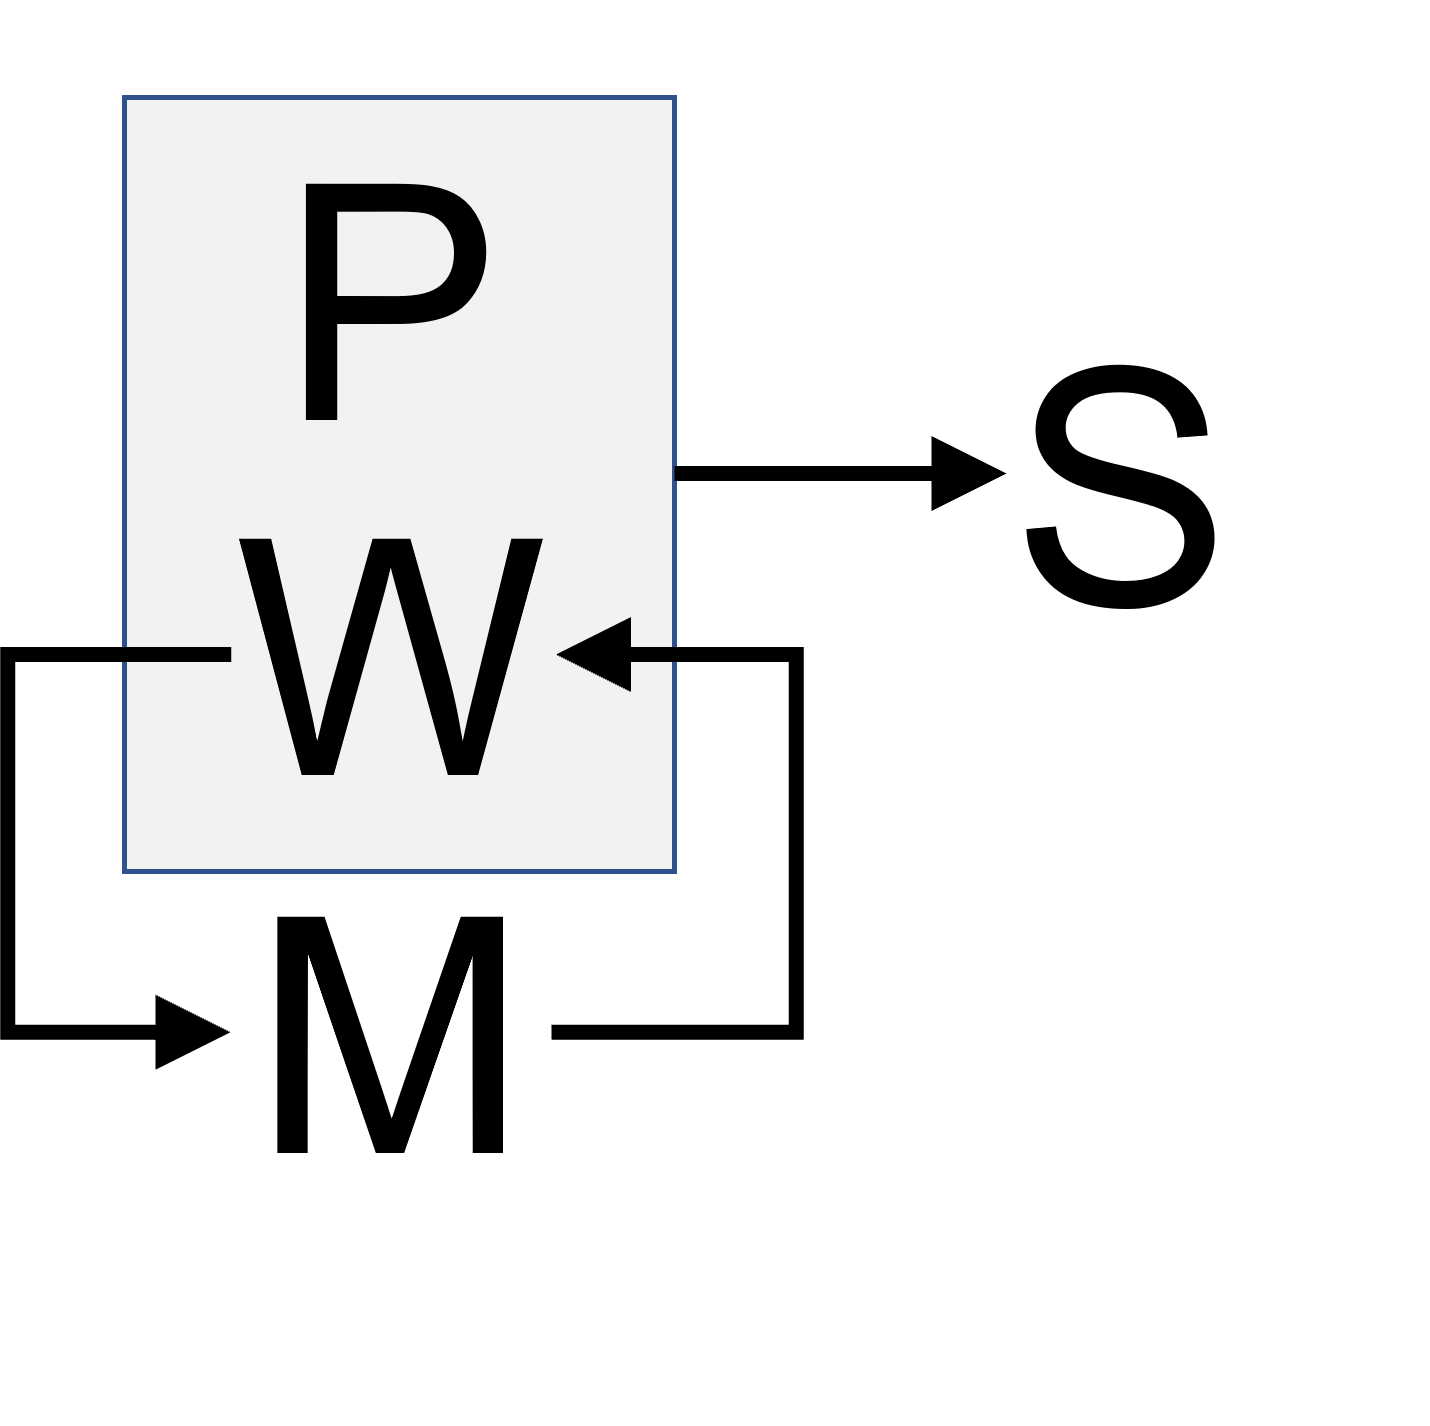
\includegraphics[width=0.2\textwidth, trim=0 0 0 0, clip]{t5/images/case1.png}
	\end{figure}\vspace{-5pt}
\end{frame}

\begin{frame}[fragile]{\boss{Extra} - Case 1 (Solution)}
	$R = \{W, M, P, S\}$\\
	$\Sigma = \{\{W\} \rightarrow \{M\}, \{M\} \rightarrow \{W\},
	\{W, P\} \rightarrow \{S\}\}$.\\\vspace{5pt}
	
	\textbf{Solution}:\\
	(1) The attribute closure of $R$ is:
	\begin{align*} 
		\Sigma^{+} = \{&\{W\}^{+} \rightarrow \{W, M\},\\
		&\{M\}^{+} \rightarrow \{W, M\},\\
		&\{P\}^{+} \rightarrow \{P\},\\
		&\{S\}^{+} \rightarrow \{S\},\\
		&\{{M,W}\}^{+} \rightarrow \{W, M\},\\
		&\{{M,P}\}^{+} \rightarrow \{W, M, P, S\},\\
		&\{{M,S}\}^{+} \rightarrow \{W, M, S\},\\
		&\{{W,P}\}^{+} \rightarrow \{W, M, P, S\},\\
		&\{{W,S}\}^{+} \rightarrow \{W, M, S\},...\}.
	\end{align*} 
	
	Now we find candidate keys: $\{W, P\}$ and $\{M, P\}$.\\
	Prime attributes: $W, M, P$
\end{frame}

\begin{frame}[fragile]{\boss{Extra} - Case 1 (Solution)}
	(2) The compact minimal cover is:\\\vspace{5pt}
	
	$\{W\} \rightarrow \{M\},$\\
	$\{M\}  \rightarrow \{W\},$\\
	$\{W, P\} \rightarrow \{S\}.$\\\vspace{5pt}
	
	(3)  Yes it is 2NF, 3NF, but not BCNF (e.g., $\{W\} \rightarrow \{M\}$, where $\{W\}$ is not a superkey).\\\vspace{5pt}
	
	(4) Omitted as it is 3NF. \\\vspace{5pt}
	
	(5) Decomposition at $\{W\} \rightarrow \{M\}$:\\\vspace{5pt}
	
	$R_1 = (\underline{W}, \underline{M}),$\\
	$R_2 = (\underline{W}, \underline{P}, S).$\\\vspace{5pt}
	
	It is (luckily) dependency preserving.
	
\end{frame}

\begin{frame}[fragile]{\boss{Extra} - Case 2}
	We are designing a transcript issuing system for our university. 
	Each student is identified by its matric number/student ID, written as $S$.
	We are going to record a grade ($G$) for each student ($S$) and each module ($M$).
	We also record students' names ($N$) and their faculty ($F$). In case any verification is needed, we also save the dean's name for each department ($D$) so that people can contact him/her.\\\vspace{10pt}
	\textbf{Questions}:\\
	(1) Find \textbf{candidate key(s)} and \textbf{prime attribute(s)} from attribute closures $\Sigma^{+}$.\\
	(2) Compute the \textbf{compact minimal cover} of $R$ with all FDs $\Sigma$.\\
	(3) Determine if it is \textbf{2NF}? If yes, is it \textbf{3NF}? If yes, is it \textbf{BCNF}?\\
	(4) If it is not 3NF, \textbf{synthesis} the relations to make it 3NF.\\
	(5) If it is not BCNF, \textbf{decomposite} the relations to make it BCNF and verify the \textbf{dependency preservation}. 
\end{frame}

\begin{frame}[fragile]{\boss{Extra} - Case 2 (Solution)}
	\textbf{S}: student ID; \textbf{M}: module; \textbf{N}: name;
	\textbf{F}: faculty; \textbf{G}: grade; \textbf{D}: dean\\\vspace{5pt}
	$R = \{S, M, G, N, F, D\}$\\
	$\Sigma = \{\{S, M\} \rightarrow \{G\}, 
	\{S\} \rightarrow \{N, F\},
	\{F\} \rightarrow \{D\}\}$.\\\vspace{15pt}
	\begin{figure}
		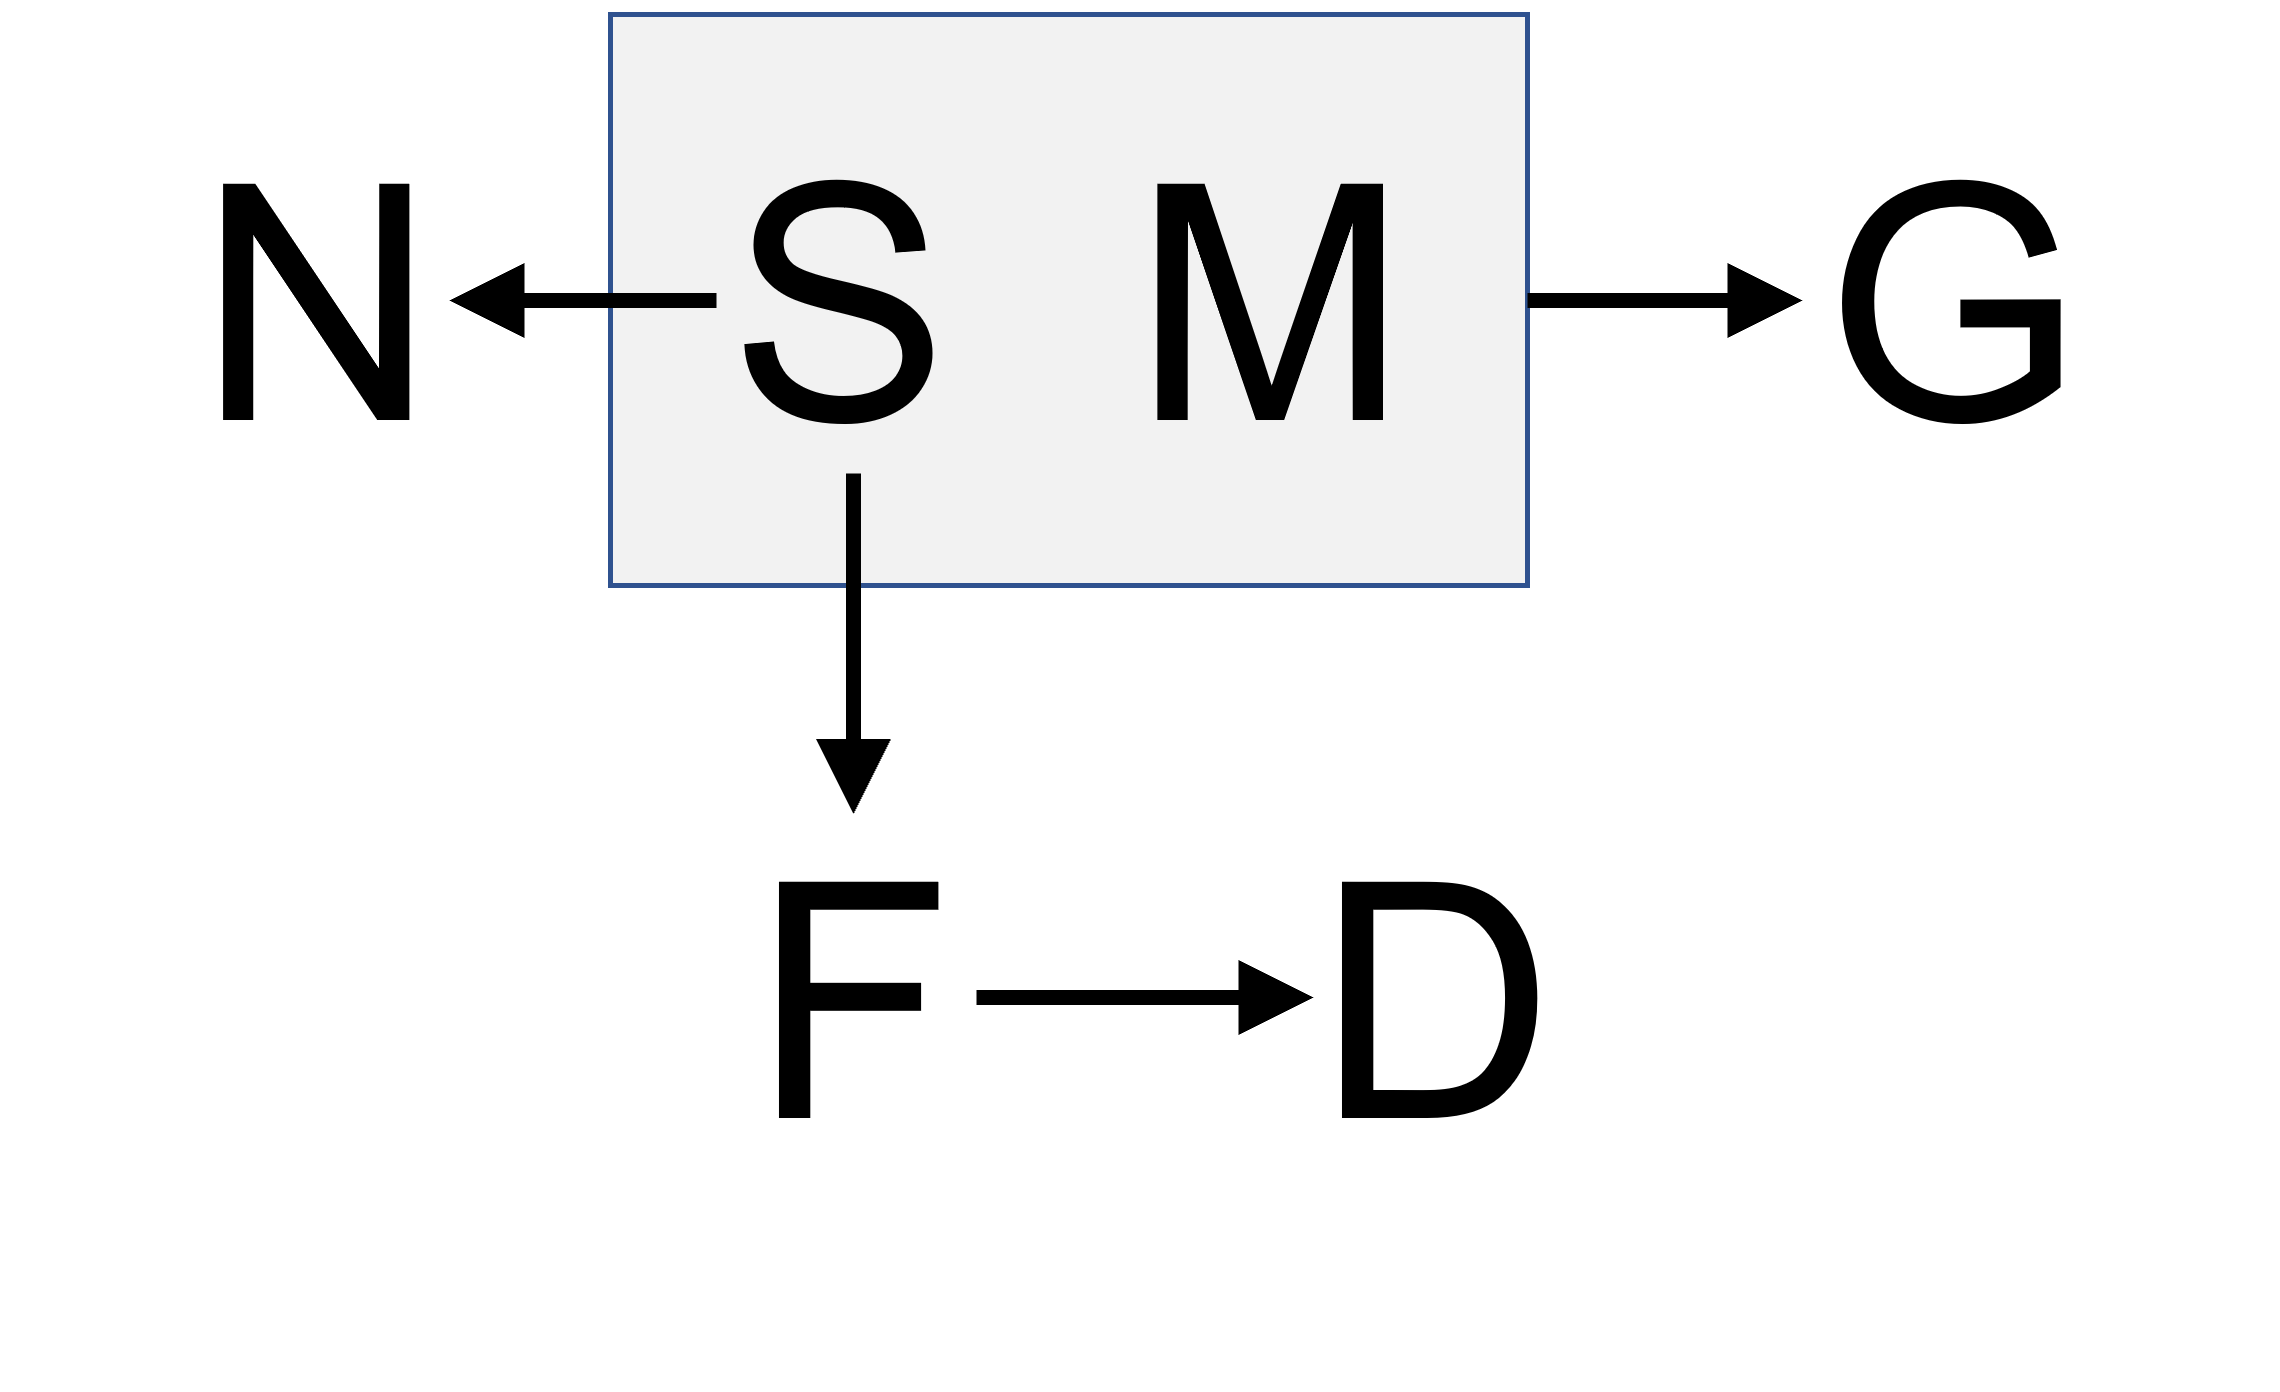
\includegraphics[width=0.4\textwidth, trim=0 0 0 0, clip]{t5/images/case2.png}
	\end{figure}\vspace{-5pt}
\end{frame}

\begin{frame}[fragile]{\boss{Extra} - Case 2 (Solution)}
	$R = \{S, M, G, N, F, D\}$\\
	$\Sigma = \{\{S, M\} \rightarrow \{G\}, 
	\{S\} \rightarrow \{N, F\},
	\{F\} \rightarrow \{D\}\}$.\\\vspace{5pt}
	
	\textbf{Solution}:\\
	(1) The attribute closure of $R$ is:
	\begin{align*} 
		\Sigma^{+} = \{&\{S\}^{+} \rightarrow \{S, N, F, D\},\\
		&\{M\}^{+} \rightarrow \{M\},\\
		&\{G\}^{+} \rightarrow \{G\},\\
		&\{N\}^{+} \rightarrow \{N\},\\
		&\{F\}^{+} \rightarrow \{F, D\},\\
		&\{D\}^{+} \rightarrow \{D\},\\
		&\{{S, M}\}^{+} \rightarrow \{S, M, N, F, D, G\},\\
		&\{{S, G}\}^{+} \rightarrow \{S, G, N, F, D\}, ...
	\end{align*} 
	
	Now we find candidate keys: $\{S, M\}$.\\
	Prime attributes: $S, M$
\end{frame}

\begin{frame}[fragile]{\boss{Extra} - Case 2 (Solution)}
	(2) The compact minimal cover is:\\\vspace{5pt}
	
	$\{S, M\} \rightarrow \{G\},$\\
	$\{S\}  \rightarrow \{N, F\},$\\
	$\{F\} \rightarrow \{D\}.$\\\vspace{5pt}
	
	(3)  No it is not 2NF (e.g., $\{S\}\rightarrow\{N, F\}$, \{N, F\} are not prime attributes and $S$ is a subset of candidate key). Therefore it is not 3NF, and not BCNF, too.\\\vspace{5pt}
	
	(4) Synthesis result has 3 relations and is (luckily) BCNF: \\\vspace{5pt}
	
	$R_1 = (\underline{S,M}, G),$\\
	$R_2 = (\underline{S}, N, F),$\\
	$R_3 = (\underline{F}, D).$\\\vspace{5pt}
	
\end{frame}

\begin{frame}[fragile]{\boss{Extra} - Case 2 (Solution)}
	(5) Decomposition at $\{F\} \rightarrow \{D\}$:\\\vspace{5pt}
	
	$R_1 = (\underline{F}, D),$\\
	$R_2 = (\underline{S}, \underline{M}, G, N, F).$\\\vspace{5pt}
	
	However, $R_2$ needs to be further decomposed, at $\{S\} \rightarrow \{N\}$:\\\vspace{5pt}
	
	$R_{2.1} = (\underline{S}, N, F).$\\
	$R_{2.2} = (\underline{S}, \underline{M}, G).$\\\vspace{5pt}
	
	As the result, the BCNF decomposition is (luckily) dependency preserving and is given below:\\\vspace{5pt}
	
	$R_1 = (\underline{F}, D),$\\
	$R_{2.1} = (\underline{S}, N, F).$\\
	$R_{2.2} = (\underline{S}, \underline{M}, G).$\\\vspace{5pt}
	
	\textit{(In fact this decomposition result is same with the synthesis one)}
\end{frame}

\begin{frame}[fragile]{\boss{Extra} - Case 3}
	This time we deal with abstract relations with functional dependencies shown as in the figure below:\\\vspace{-5pt}
	
	\begin{figure}
		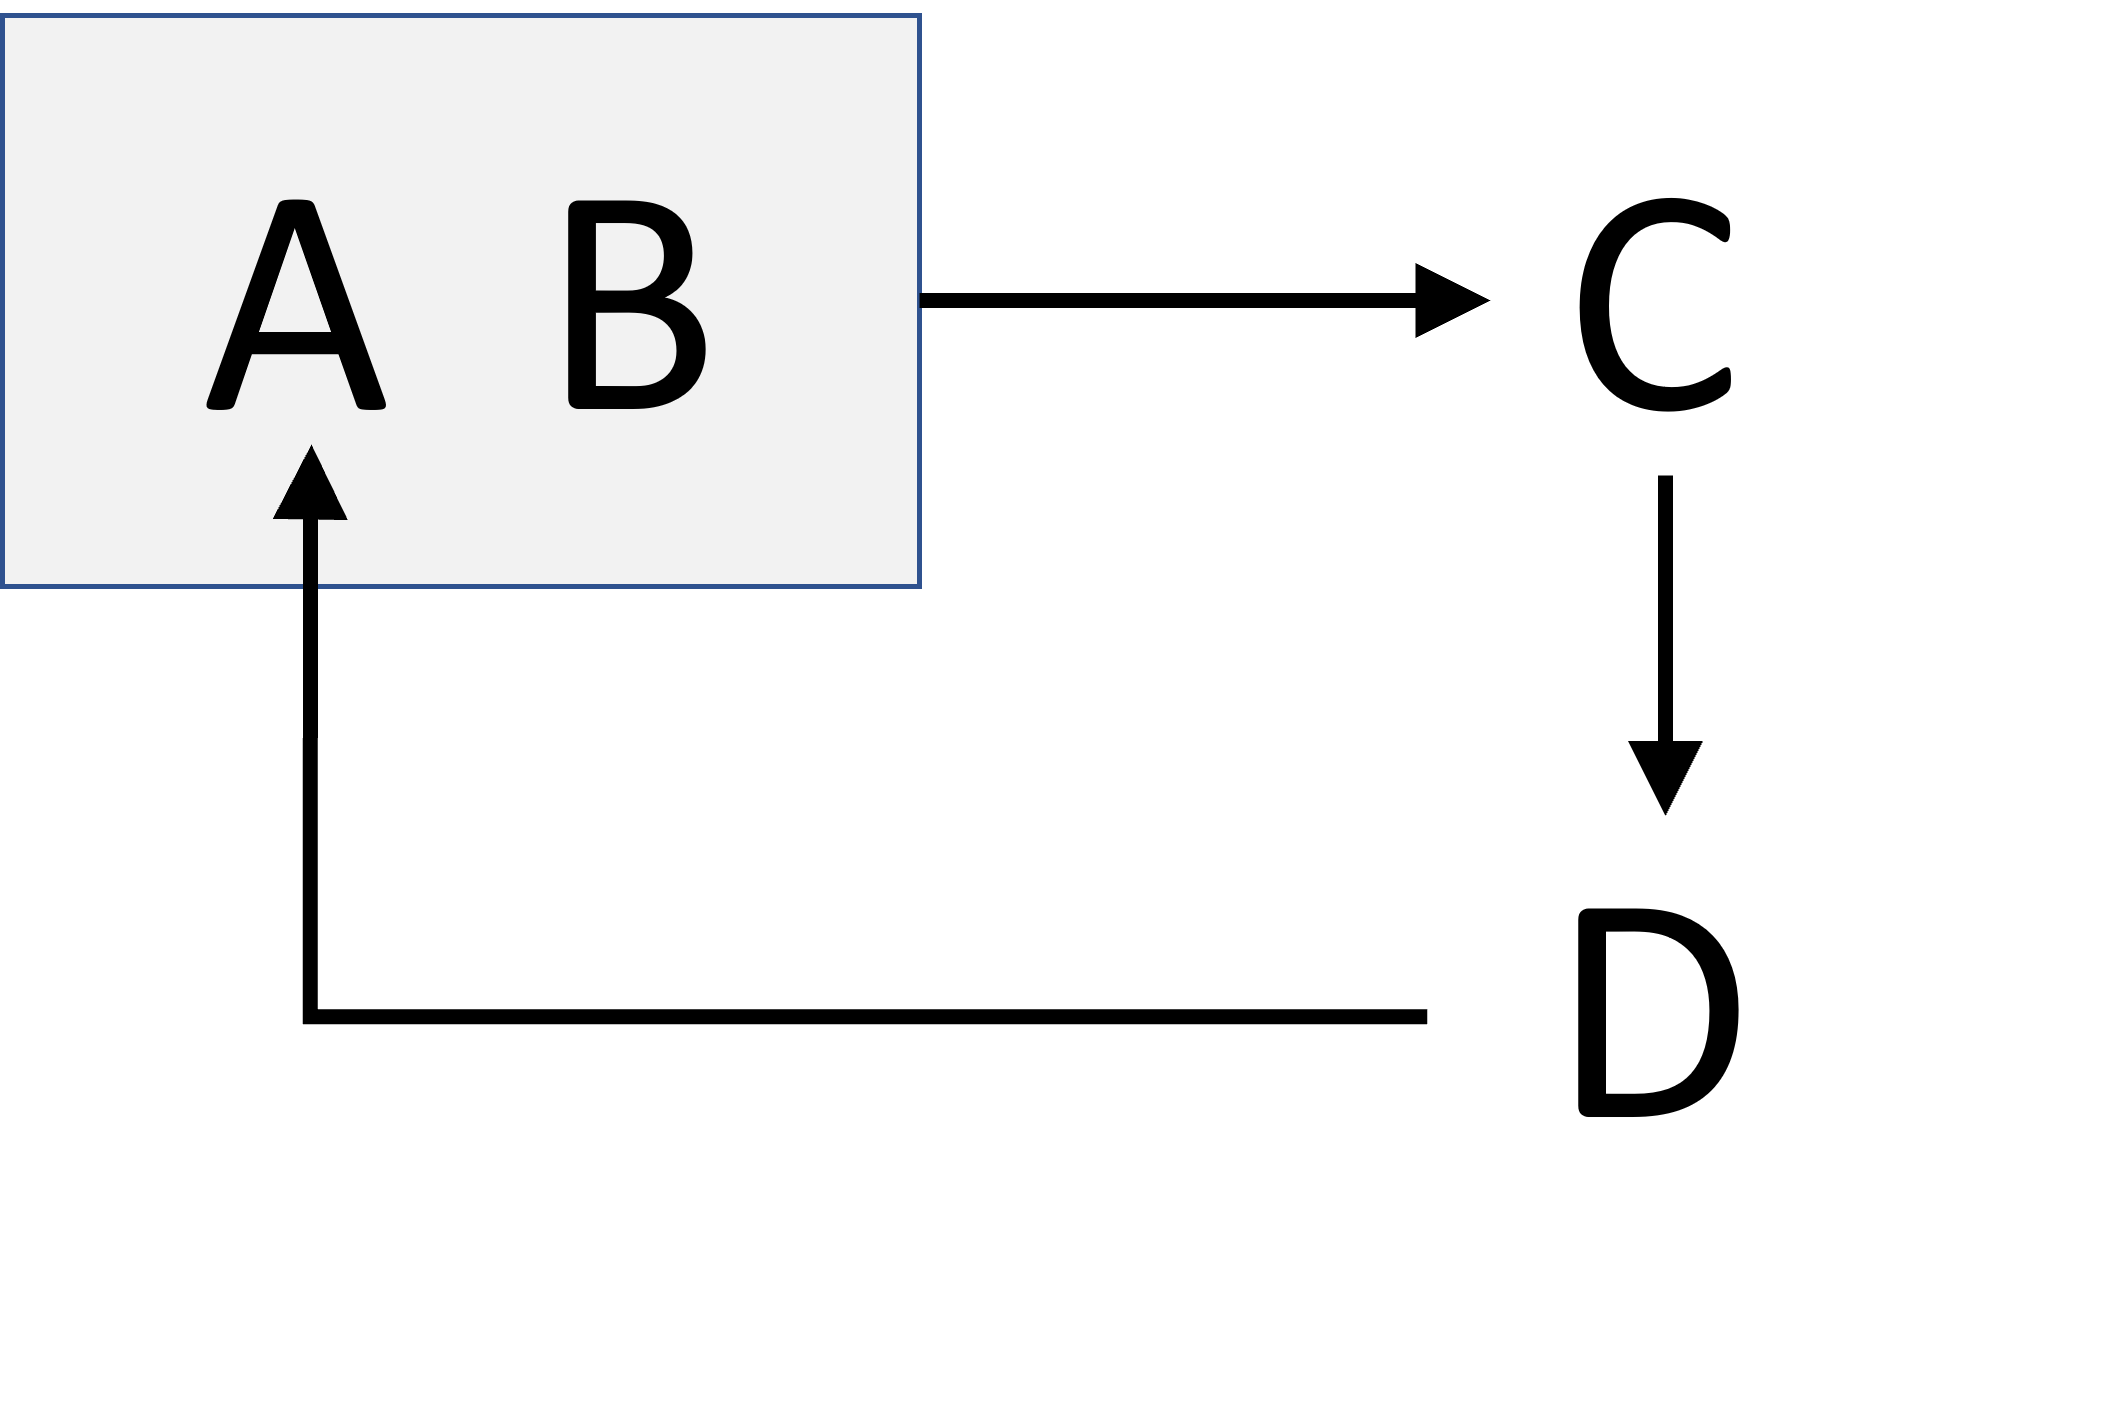
\includegraphics[width=0.4\textwidth, trim=0 0 0 0, clip]{t5/images/case3.png}
	\end{figure}\vspace{-10pt}
	
	\textbf{Questions}:\\
	(1) Find \textbf{candidate key(s)} and \textbf{prime attribute(s)} from attribute closures $\Sigma^{+}$.\\
	(2) Compute the \textbf{compact minimal cover} of $R$ with all FDs $\Sigma$.\\
	(3) Determine if it is \textbf{2NF}? If yes, is it \textbf{3NF}? If yes, is it \textbf{BCNF}?\\
	(4) If it is not 3NF, \textbf{synthesis} the relations to make it 3NF.\\
	(5) If it is not BCNF, \textbf{decomposite} the relations to make it BCNF and verify the \textbf{dependency preservation}. 
\end{frame}


\begin{frame}[fragile]{\boss{Extra} - Case 3 (Solution)}
	
	\textbf{Solution}:\\
	(1) The attribute closure of $R = \{A, B, C, D\}$ is:\\\vspace{5pt}
	\begin{scriptsize}
		\begin{align*} 
			\Sigma^{+} = \{&\{A\}^{+} \rightarrow \{A\},\\
			&\{B\}^{+} \rightarrow \{B\},\\
			&\{C\}^{+} \rightarrow \{A, C, D\},\\
			&\{D\}^{+} \rightarrow \{A, D\},\\
			&\{A, B\}^{+} \rightarrow \{A, B, C, D\},\\
			&\{A, C\}^{+} \rightarrow \{A, C, D\},\\
			&\{A, D\}^{+} \rightarrow \{A, D\},\\
			&\{B, C\}^{+} \rightarrow \{A, B, C, D\}\\
			&\{B, D\}^{+} \rightarrow \{A, B, C, D\}, ...
		\end{align*}
	\end{scriptsize}
	
	Now we find candidate keys: $\{A, B\}$ or $\{B, C\}$ or $\{B, D\}$.\\
	Prime attributes: $A, B, C, D$ (There is no non-prime attribute for this case)
\end{frame}

\begin{frame}[fragile]{\boss{Extra} - Case 3 (Solution)}
	(2) The compact minimal cover is:\\\vspace{5pt}
	
	$\{A, B\} \rightarrow \{C\}$\\
	$\{C\} \rightarrow \{D\}$\\
	$\{D\} \rightarrow \{A\}$.\\\vspace{5pt}
	
	(3) Yes it is 2NF and 3NF (because all attributes are prime attributes). However, it is not BCNF (e.g., $\{C\} \rightarrow \{D\}$ and $\{D\} \rightarrow \{A\}$).\\\vspace{5pt}
	
	(4) Omitted as it is 3NF. \\\vspace{5pt}
	
\end{frame}

\begin{frame}[fragile]{\boss{Extra} - Case 3 (Solution)}
	(5) Decomposition at $\{C\} \rightarrow \{D\}$:\\\vspace{3pt}
	
	$R_1 = (A, \underline{C}, D),$\\
	$R_2 = (\underline{B}, \underline{C}).$\\\vspace{3pt}
	
	The $R_1$ is not in BCNF (e.g., $\{D\} \rightarrow \{A\}$), let's further decompose it:\\
	$R_{1.1} = (A, \underline{D}),$\\
	$R_{1.2} = (\underline{C}, D),$\\\vspace{3pt}
	
	In this way all 3 relations ($R_{1.1}$, $R_{1.2}$ and $R_{2}$) are BCNF, but we lose a dependency $\{A, B\} \rightarrow \{C\}$.\\\vspace{10pt}
	
	\textcolor{red}{How about we change the entry point of decomposition?}\\\vspace{3pt}
	
	Decomposition at $\{D\} \rightarrow \{A\}$:\\\vspace{3pt}
	
	$R_1 = (A, \underline{D}),$\\
	$R_2 = (B, \underline{C}, D).$\\\vspace{5pt}
	
	In this way both relations are BCNF, but we (still) lose that dependency $\{A, B\} \rightarrow \{C\}$.
\end{frame}

\begin{frame}[fragile]{\boss{Extra} - Case 4}
	Another abstract relations with functional dependencies shown as in the figure below:\\\vspace{-5pt}
	
	\begin{figure}
		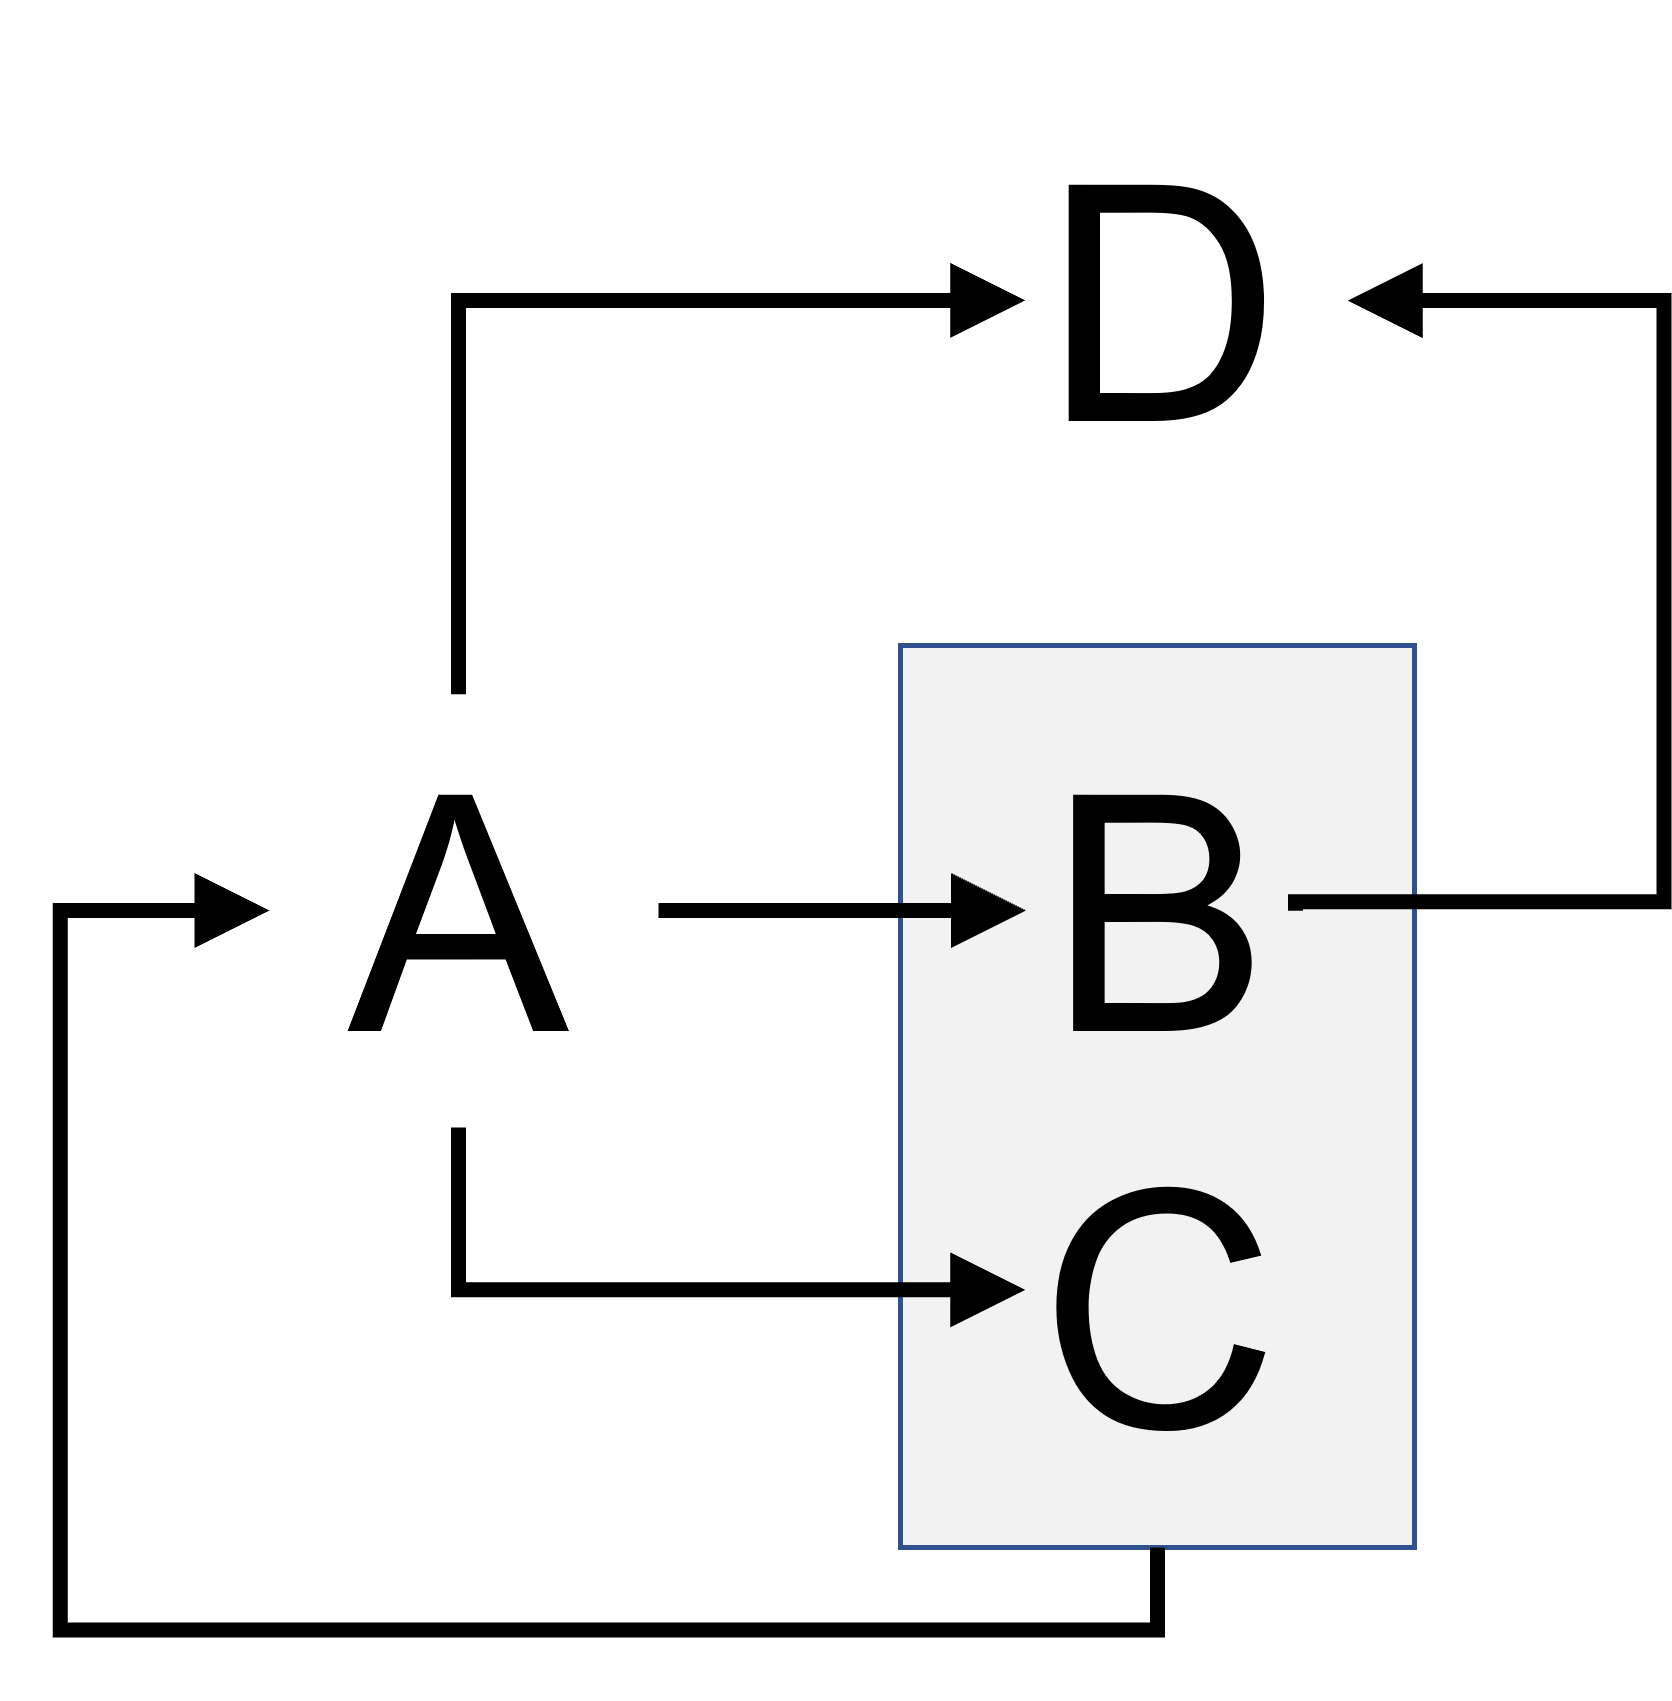
\includegraphics[width=0.25\textwidth, trim=0 0 0 0, clip]{t5/images/case4.png}
	\end{figure}\vspace{-5pt}
	
	\textbf{Questions}:\\
	(1) Find \textbf{candidate key(s)} and \textbf{prime attribute(s)} from attribute closures $\Sigma^{+}$.\\
	(2) Compute the \textbf{compact minimal cover} of $R$ with all FDs $\Sigma$.\\
	(3) Determine if it is \textbf{2NF}? If yes, is it \textbf{3NF}? If yes, is it \textbf{BCNF}?\\
	(4) If it is not 3NF, \textbf{synthesis} the relations to make it 3NF.\\
	(5) If it is not BCNF, \textbf{decomposite} the relations to make it BCNF and verify the \textbf{dependency preservation}. 
\end{frame}

\begin{frame}[fragile]{\boss{Extra} - Case 4 (Solution)}
	
	\textbf{Solution}:\\
	(1) The attribute closure of $R = \{A, B, C, D\}$ is:\\
	\begin{scriptsize}
		\begin{align*} 
			\Sigma^{+} = \{&\{A\}^{+} \rightarrow \{A, B, C, D\},\\
			&\{B\}^{+} \rightarrow \{B, D\},\\
			&\{C\}^{+} \rightarrow \{C\},\\
			&\{D\}^{+} \rightarrow \{D\},\\
			&\{A, B\}^{+} \rightarrow \{A, B, C, D\},\\
			&\{A, C\}^{+} \rightarrow \{A, B, C, D\} (trivial),\\
			&\{A, D\}^{+} \rightarrow \{A, B, C, D\} (trivial),\\
			&\{B, C\}^{+} \rightarrow \{A, B, C, D\}\\
			&\{B, D\}^{+} \rightarrow \{B, D\}, ...
		\end{align*}
	\end{scriptsize}\vspace{-15pt}
	
	Now we find candidate keys: $\{A\}$ or $\{B, C\}$.\\
	\textcolor{brown}{Although $\{A\}\rightarrow\{B, C\}$, both of them are candidate keys because (1) their closures functionally determine all attributes of $R$; (2) both of them are minimal superkeys (cannot be further simplified).}\\
	Prime attributes: $A, B, C$.
\end{frame}

\begin{frame}[fragile]{\boss{Extra} - Case 4 (Solution)}
	\textcolor{red}{\textbf{\hl{Updated version (an error raised in class corrected)}}}\\
	(2) First let's list all FDs given in the question:\\\vspace{5pt}
	$\{A\} \rightarrow \{B,C,D\}$, 
	$\{B\} \rightarrow \{D\}$, 
	$\{B, C\} \rightarrow \{A\}$.\\\vspace{5pt}
	
	Step 1: Simplify the RHS:\\\vspace{5pt}
	$\{A\} \rightarrow \{B\}$\\
	$\{A\} \rightarrow \{C\}$\\
	$\{A\} \rightarrow \{D\}$\\
	$\{B\} \rightarrow \{D\}$\\
	$\{B, C\} \rightarrow \{A\}$.\\\vspace{5pt}
	
	Step 2: Simplify the LHS \\
	(There is only 1 FD with multiple attributes on the LHS and that FD cannot be simplified as there does not exist any FD implies $A$) \\\vspace{5pt}
	
\end{frame}

\begin{frame}[fragile]{\boss{Extra} - Case 4 (Solution)}
	Step 3: Simplify the set:\\\vspace{5pt}
	
	$\{A\} \rightarrow \{B\}$\\
	$\{A\} \rightarrow \{C\}$\\
	$\cancel{\{A\} \rightarrow \{D\}}$ (because $\{A\} \rightarrow \{B\}$ and $\{B\} \rightarrow \{D\}$)\\
	$\{B\} \rightarrow \{D\}$\\
	$\{B, C\} \rightarrow \{A\}$.\\\vspace{5pt}
	
	Finally, the compact minimal cover is:\\\vspace{5pt}
	
	$\{A\} \rightarrow \{B, C\}$\\
	$\{B\} \rightarrow \{D\}$\\
	$\{B, C\} \rightarrow \{A\}$.\\\vspace{5pt}
	
\end{frame}

\begin{frame}[fragile]{\boss{Extra} - Case 4 (Solution)}
	(3) No it is not 2NF (e.g., $\{B\} \rightarrow \{D\}$, where $D$ is a non-prime attribute but $B$ is a subset of candidate key). Therefore, it is not 3NF and not BCNF, too. (all because of $\{B\} \rightarrow \{D\}$)\\\vspace{5pt}
	
	
	\textcolor{red}{\textbf{\hl{Updated version (an error raised in class corrected)}}}\\
	(4) Synthesis result has 2 relations and each one is (luckily) BCNF: \\\vspace{5pt}
	
	$R_1 = (\underline{A}, \underline{B, C}),$\\\vspace{2pt}
	$R_2 = (\underline{B}, D),$\\\vspace{1pt}
	$\cancel{R_3 = (\underline{B, C}, \underline{A})}.$ (duplicate with $R_1$)\\\vspace{5pt}
	
\end{frame}

\begin{frame}[fragile]{\boss{Extra} - Case 4 (Solution)}
	\textcolor{red}{\textbf{\hl{Updated version (an error raised in class corrected)}}}\\
	(5) Decomposition at $\{B\} \rightarrow \{D\}$:\\\vspace{5pt}
	
	$R_1 = (\underline{B}, D),$\\
	$R_2 = (\underline{A}, \underline{B, C}).$\\\vspace{5pt}
	
	In this way both relations are BCNF, and luckily we obtain the exact same result as the 3NF synthesis, therefore it is dependency preserving.\\\vspace{5pt}
	
\end{frame}

\begin{frame}[fragile]{\boss{Extra} - In-class Case 1}
	Given a relation $R=\{A, B, C\}$ with functional dependency set:\\ 
	$\Sigma=\{\{A\} \rightarrow \{B\},\{B\} \rightarrow \{C\}, \{A, B\} \rightarrow \{C\},\{B, C\} \rightarrow \{A\}\}.$\\\vspace{10pt}
	\textbf{Questions}:\\
	(1) Find \textbf{candidate key(s)} and \textbf{prime attribute(s)} from attribute closures $\Sigma^{+}$.\\
	(2) Compute the \textbf{compact minimal cover} of $R$ with all FDs $\Sigma$.\\
	(3) Determine if it is \textbf{2NF}? If yes, is it \textbf{3NF}? If yes, is it \textbf{BCNF}?\\
	(4) If it is not 3NF, \textbf{synthesis} the relations to make it 3NF.\\
	(5) If it is not BCNF, \textbf{decomposite} the relations to make it BCNF and verify the \textbf{dependency preservation}. 
\end{frame}

\begin{frame}[fragile]{\boss{Extra} - In-class Case 1 (Solution)}
	$R=\{A, B, C\}$\\ 
	$\Sigma=\{\{A\} \rightarrow \{B\},\{B\} \rightarrow \{C\}, \{A, B\} \rightarrow \{C\},\{B, C\} \rightarrow \{A\}\}.$\\\vspace{5pt}
	
	\textbf{Solution}:\\
	(1) The attribute closure of $R$ is:
	\begin{align*} 
		\Sigma^{+} = \{&\{A\}^{+} \rightarrow \{A,B,C\},\\
		&\{B\}^{+} \rightarrow \{A,B,C\},\\
		&\{C\}^{+} \rightarrow \{C\},\\
		&\{A,B\}^{+} \rightarrow \{A,B,C\},\\
		&\{A,C\}^{+} \rightarrow \{A,B,C\},\\
		&\{B,C\}^{+} \rightarrow \{A,B,C\},\\
		&\{A,B,C\}^{+} \rightarrow \{A,B,C\}\}.
	\end{align*} 
	
	Now we find candidate keys: $\{A\}$ and $\{B\}$.\\
	Prime attributes: $A, B$
\end{frame}

\begin{frame}[fragile]{\boss{Extra} - In-class Case 1 (Solution)}
	$\Sigma=\{\{A\} \rightarrow \{B\},\{B\} \rightarrow \{C\}, \{A, B\} \rightarrow \{C\},\{B, C\} \rightarrow \{A\}\}.$\\\vspace{25pt}
	
	(2) The minimal cover is:\\\vspace{5pt}
	
	$\{A\} \rightarrow \{B\},$\\
	$\{B\}  \rightarrow \{C\},$\\
	$\{B,C\} \rightarrow \{A\}.$\\\vspace{5pt}
	
	This is the compact minimal cover, too.\\\vspace{5pt}
	
	(3)  Yes it is 2NF, 3NF, and BCNF, too.\\\vspace{5pt}
	
	(4) Omitted as it is 3NF. \\\vspace{5pt}
	
	(5) Omitted as it is BCNF. \\\vspace{5pt}
	
\end{frame}

\begin{frame}[fragile]{\boss{Extra} - In-class Case 2}
	Given a relation $R=\{A, B, C, D, E\}$ with functional dependency set:\\ 
	$\Sigma=\{\{C,D\} \rightarrow \{E\},\{A,B\} \rightarrow \{B\}, \{A,C,D\} \rightarrow \{E\},\{A\} \rightarrow \{E\},\{D,E\} \rightarrow \{B,C\},\{A\} \rightarrow \{A\}\}.$\\\vspace{10pt}
	\textbf{Questions}:\\
	(1) Find \textbf{candidate key(s)} and \textbf{prime attribute(s)} from attribute closures $\Sigma^{+}$.\\
	(2) Compute the \textbf{compact minimal cover} of $R$ with all FDs $\Sigma$.\\
	(3) Determine if it is \textbf{2NF}? If yes, is it \textbf{3NF}? If yes, is it \textbf{BCNF}?\\
	(4) If it is not 3NF, \textbf{synthesis} the relations to make it 3NF.\\
	(5) If it is not BCNF, \textbf{decomposite} the relations to make it BCNF and verify the \textbf{dependency preservation}. 
\end{frame}

\begin{frame}[fragile]{\boss{Extra} - In-class Case 2 (Solution)}
	$\Sigma=\{\{C,D\} \rightarrow \{E\},\{A,B\} \rightarrow \{B\}, \{A,C,D\} \rightarrow \{E\},\{A\} \rightarrow \{E\},\{D,E\} \rightarrow \{B,C\},\{A\} \rightarrow \{A\}\}.$\\\vspace{5pt}
	
	\textbf{Solution}:\\
	\textcolor{red}{\textbf{\hl{Updated version (an error raised in class corrected)}}}\\
	(1) The attribute closure of $R$ is:
	\vspace{-10pt}\begin{columns}
	\column{0.3\textwidth}
	\begin{scriptsize}\begin{align*} 
		\Sigma^{+} = \{&\{A\}^{+} \rightarrow \{A,E\},\\
		&\{B\}^{+} \rightarrow \{B\},\\
		&\{C\}^{+} \rightarrow \{C\},\\
		&\{D\}^{+} \rightarrow \{D\},\\
		&\{E\}^{+} \rightarrow \{E\},\\
		&\{A,B\}^{+} \rightarrow \{A,B,E\},\\
		&\{A,C\}^{+} \rightarrow \{A,C,E\},\\
		&\{A,D\}^{+} \rightarrow \{A,B,C,D,E\},\\
		&\{A,E\}^{+} \rightarrow \{A,B,E\}\}\\
		& ...\\
		&\{A,C,D,E\}^{+} \rightarrow \{A,B,C,D,E\}\}\\
		&\{A,B,C,D,E\}^{+} \rightarrow \{A,B,C,D,E\}\}.
	\end{align*}\end{scriptsize} 
	
	\column{0.65\textwidth}
	\textbf{Hint}:\\
	After removing all trivial FDs, we find $A$ and $D$ have never appeared in the right-hand side, which means the candidate key must contains $A$ and $D$. We just need to find the minimal set that implies $\{B,C,E\}$. (Luckily both $A$ and $D$ together can determine $\{B,C,E\}$)\\\vspace{10pt}

	Then we can find candidate key: $\{A,D\}$. And the prime attributes: $A, D$
	\end{columns}
	
\end{frame}

\begin{frame}[fragile]{\boss{Extra} - In-class Case 2 (Solution)}
	$\Sigma=\{\{C,D\} \rightarrow \{E\},\{A,B\} \rightarrow \{B\}, \{A,C,D\} \rightarrow \{E\},\{A\} \rightarrow \{E\},\{D,E\} \rightarrow \{B,C\},\{A\} \rightarrow \{A\}\}.$\\\vspace{5pt}
	
	(2) The compact minimal cover is:\\\vspace{5pt}
	
	\begin{columns}
	\column{0.35\textwidth}
	$\{C,D\} \rightarrow \{E\},$\\
	$\cancel{\{A,B\} \rightarrow \{B\}}$,\\
	$\cancel{\{A,C,D\} \rightarrow \{E\}}$,\\
	$\{A\}  \rightarrow \{E\},$\\
	$\{D,E\} \rightarrow \{B\}.$\\
	$\{D,E\} \rightarrow \{C\}.$\\
	$\cancel{\{A\} \rightarrow \{A\}}$\\\vspace{5pt}
	\column{0.05\textwidth} $\rightarrow$
	\column{0.45\textwidth}
	So the finalized set is:\\
	$\{C,D\} \rightarrow \{E\},$\\
	$\{A\}  \rightarrow \{E\},$\\
	$\{D,E\} \rightarrow \{B, C\}.$
	\end{columns}
	
	\textcolor{red}{\textbf{\hl{Updated version (an error raised in class corrected)}}}\\
	(3)  Yes it is in 2NF. But not in 3NF, and not in BCNF, too.\\\vspace{5pt}
	
	E.g., $\{C,D\} \rightarrow \{E\}$ is not trivial, the LHS is not a superkey and the RHS is not a prime attribute, therefore it violates 3NF (in fact all four FDs in the compact minimal cover violate 3NF and BCNF).
	
\end{frame}


\begin{frame}[fragile]{\boss{Extra} - In-class Case 2 (Solution)}
	\textcolor{red}{\textbf{\hl{Updated version (an error raised in class corrected)}}}\\
	(4) Recall the compact minimal cover:\\\vspace{5pt}
	
	$\{C,D\} \rightarrow \{E\},$
	$\{A\}  \rightarrow \{E\},$
	$\{D,E\} \rightarrow \{B,C\}.$\\\vspace{5pt}
	
	Let's do 3NF synthesis:\\ \vspace{5pt}
	\begin{columns}
	\column{0.55\textwidth}
	$R_1 = (\underline{C, D}, E),$\\
	$R_2 = (\underline{A}, E),$\\
	$R_3 = (B, C, \underline{D, E}).$\\\vspace{3pt}
	(The candidate key is not included in any relation fragment above, so we add a new fragment manually)\\\vspace{3pt}
	$R_4 = (\underline{A, D}).$\\\vspace{3pt}
	
	\column{0.02\textwidth} $\rightarrow$
	\column{0.3\textwidth}
	So the simplified result is:\\
	($R_1$ can be subsumed in $R_3$)
	$R_2 = (\underline{A}, E),$\\
	$R_3 = (B, \underline{C,D,E}),$\\
	$R_4 = (\underline{A, D}),$\\
	All 3 fragments are in BCNF.
	
	\end{columns}

\end{frame}

\begin{frame}[fragile]{\boss{Extra} - In-class Case 2 (Solution)}
	\textcolor{red}{\textbf{\hl{Updated version (an error raised in class corrected)}}}\\
	(5) Recall the compact minimal cover:\\
	
	$\{C,D\} \rightarrow \{E\},$\\
	$\{A\}  \rightarrow \{E\},$\\
	$\{D,E\} \rightarrow \{B,C\}.$\\\vspace{5pt}
	
	Decomposition at $\{C,D\} \rightarrow \{E\}$:\\\vspace{5pt}
		
	$R_1 = (\underline{C,D}, E),$\\
	$R_2 = (\underline{A}, B, \underline{C,D}).$\\\vspace{5pt}
	
	We can find that:\\\vspace{5pt}
	$\Sigma_1 = \{\{C,D\}\rightarrow\{E\}\}$\\
	$\Sigma_2 = \emptyset$
	
	Both relations are BCNF\\\vspace{5pt}
	However, we lose lots of dependency in this decomposition. E.g., $\{A\}\rightarrow\{E\}, \{D,E\}\rightarrow\{B,C\}$.
\end{frame}

\begin{frame}{}
	\centering  
	For any further question, please feel free to email me:\vspace{10pt}
	
	huasong.meng@u.nus.edu\\\vspace{3pt}
	
	\begin{tcolorbox}
		\begin{center}
			\textcolor{red}{Copyright 2021 Mark H. Meng. All rights reserved.}
		\end{center}
	\end{tcolorbox}
\end{frame}